%%%%%%%%%%%%%%%%%%%%%%%%%%%%%%%%%%%%%%%%%%%%%%%%%%%%%%%%%%%%%%%%%%%
%Conc_Ventilateur.tex : Projet de conception - Contrôle Arduino d'un Ventilateur | Électronique et mesures expérimentales GPH-2006, Physique électronique PHY-2002 | Département de physique, de génie physique et d'optique - FSG - Université Laval
%------------------------------------------------------------------
%Créé par Jérémie Guilbert, Louis-Philippe Dallaire & Marc-André Vigneault
%Contributions par Claudine Nì. Allen
%Compilateur pdfLaTeX, distribution TeX Live 2022
%Dernière modification CA : 22 novembre 2022
%
%%%ToDo
%
% - Pratiquement tout le monde conçoit totalement par essai-erreur, comment forcer des calculs "back of the envelope" avant de "tomber" dans les outils de simulation numérique et ECAD/EDA?
%
% - Les deux dernières grosses difficulté hardware sont 1) le moteur n'a d'encodeur retournant la mesure de vitesse (pourra être acheté sur Adafruit ou autre inspiré des composants Fritzing ou TinkerCAD) et plus compliqué 2) Source de lumière calibrée et alignée pour reproduire une illumination maximale identique sur les photorésistances de toutes les équipes difficile à implémenter pour nous au labo. Les parties sur le max de luminosité possible (slider Tinkercad notamment) sont donc commentées out. Voir s'il y a lieu de ramener ou pas éventuellement, mais à plus court terme, clarifier la bouette d'étalonnage: même Tinkercad n'a qu'un vague slider de luminosité, ce pkoi le graphe d'optimisation est demandé en fonction de la photorésistance et non pas de la luminosité, mais ce n'est malheureusement pas "catché" par toutes les équipes.
%
% - J'ai beaucoup de commentaires à l'intérieur du texte ci-dessous, tout relire et modifier selon comment ça va dans l'adaptation au mode hybride de retour post-pandémie.
%
% - Éventuellement, intégrer l'annexe dans les compléments dont un nouveau spécifique à l'Arduino. Y mettre une à la fin de ce dernier à partir des ressources Arduino préférees des étudiants, à voter sur Teams. Développer un/des compléments séparés (éliminer l'annexe éventuellement) et/ou capsules vidéo à pour les outils des ateliers et ce projet: Arduino (la carte et le IDE), Fritzing, Tinkercad, Falstad(possiblement bien avant dans les cours asynchrones avec ce dernier). Mentionner seulement dans la section logiciel du site de cours (pas matériel didactique obligatoire) et aborder plus au cours 6 présentiel qui traite entre autres de la 2e partie de la session.
%
%%%%%%%%%%%%%%%%%%%%%%%%%%%%%%%%%%%%%%%%%%%%%%%%%%%%%%%%%%%%%%%%%%%%

\RequirePackage[l2tabu, orthodox]{nag} %%Check for obsolete commands
\documentclass[english,french,12pt]{article}
%
%----------------------------------------------------------------
%### Loading Packages ###
%
%## Encoding, Typography & Language ##
\usepackage[utf8]{inputenc}
\usepackage[T1]{fontenc}
\usepackage{babel} %%is globally set to French, switch to English by inverting order in the '\documentclass' options
\usepackage{lmodern,csquotes} %%extended support for proper typesetting of accented letters & quotes with '\textquote{}' and the '\begin{displayquote}...\end{displayquote}' environment
\PassOptionsToPackage{mathscr}{eucal}\usepackage{amsfonts,eucal,mathrsfs,textcomp} %%math fonts and more symbols, extensively listed in the 'latex-AllSymbolList.pdf' of the 'Templates_labOMC' repo
\usepackage{ulem} %%underlining with '\uline{}', '\uwave{}' etc. and strikeout with '\sout{}'
\normalem
%\usepackage{newtxtext} %%for a Times New Roman text font output.

%## Colors, Boxes & Figures ##
\usepackage[usenames,x11names,table]{xcolor} %%colour names in 'xcolor-palettes.pdf' of the 'Templates_labOMC' repo. For printing, the [cmyk,dvipsnames] colour model is preferred.
%\usepackage{fancybox} %%more framed boxes
%\usepackage[breakable]{tcolorbox} %%coloured boxes with optional title
%\usepackage{float} %%more control on any floating environments 
%\usepackage{array,dcolumn,tabularx,multirow,longtable,booktabs} %%more control of 'tabular' and 'array' environments
\usepackage{graphicx,wrapfig,caption,sidecap} %%compiling with 'pdfLaTeX' supports .pdf,.pdf_tex .png, .jpg and .eps(indirectly) files. %Use '\includeinkscape' for .pdf_tex files exported from Inkscape or convert directly to TiKZ code with the 'svg2tikz' extension.

%## Maths & Physics ##
\usepackage{amsmath,amsthm,amssymb}
%\usepackage{cancel,trfsigns} %%math simplifications & signs for transforms respectively
%\usepackage[all]{xy} %%nice math diagrams
\usepackage{siunitx} %scientific & complex numbers, measurement & uncertainty, see 'latex-SIunitx.pdf' in the 'Templates_labOMC' repo.
\usepackage{physics} %typesetting for mathematical physics, see 'latex-PhysicsPack.pdf' in the 'Templates_labOMC' repo.
\usepackage{pgfplots} %graphs of symbolic functions and equations
%\usepackage{tikz-network} %%crystal lattice & complex networks drawing
%\usepackage{tikz-optics} %%optical drawing
%\usepackage{pstricks,pst-optexp,pst-optic} %%neat PSTricks optical drawing
%\usepackage{tikzorbital,chemfig,chemmacros,mhchem} %%chemical drawings/diagrams and formulae & safety
%\usepackage{pstricks,pst-labo} %%laboratory chemical glassware
%\usepackage{pstricks,dsptricks,pst-sigsys} %%signal processing plots/drawings
%\usepackage[RPvoltages,americanvoltages,americancurrents]{circuitikz} %%electrical circuit drawing with Rising Potential voltages
%\usetikzlibrary{babel} %%needed for electrical circuit drawing when running babel-french
%\usepackage{yquant} %%quantum circuit drawing

%## Miscellaneous Nice Tools ##
\usepackage{ccicons} %%Creative Commons icons, reusable content at <https://search.creativecommons.org/>
%\usepackage{media9,animate,tikz} %%tools for multimedia and general drawing
%\usepackage{pythontex} %%runs Python code in the LaTeX source files and typeset the output

%## Bibliography ##
%\usepackage[backend=biber,sorting=none]{biblatex} %%see 'cheatsheet-BibLaTeX.tex' in the 'Templates_labOMC' repo.
%\addbibresource{} %%import your .bib file in BibLaTeX format from Zotero

%## Hyperlinks ##
\usepackage{hyperref,xurl} %%'\href{_URL_}{_hypertext_}' to link the hypertext & '\url{_URL_}' to link the displayed web address, each internal '~\ref{_label_}' is also hyperlinked ; xurl for more line breaks.
\usepackage{doi} %%automatically resolves object identifiers such as IDs from doi, arXiv, OCLC, etc., use '\doi{}' if the former bugs.

%## Layout ##
%%Watch for conflicts with the overall document class.
\usepackage{geometry} %%page layout
\usepackage{fancyhdr}
\usepackage{setspace} %%interline spacing tools ; unit relative to current font: em ~width of an 'M' (uppercase), typically equal to the font size in pt
\usepackage{enumitem} %%tools to change list format
\usepackage{import}
%\usepackage{tasks,xsim,epigraph,boxedminipage,multicol,lscape,rotating,makeidx,showidx,glossaries}

%---------------------------------------------------------
%### Settings ###
%
%## Configuring the layout and other format setups ##
%\the\parindent{}, \the\value{equation} %%and other '\the' commands to see the current parameter, counter,... value
\geometry{  %%for geometry package
%    showframe,  %%uncomment to see lines delimiting the dimension boxes
    letterpaper,
    margin=0.75in}
\pagestyle{fancy}
\fancyhf{}
\renewcommand{\headrulewidth}{0pt}
\fancyfoot[C]{-\thepage-} %%bottom center page numbering
%\interfootnotelinepenalty=10000 %%uncomment if long footnotes are incorrectly spreading on several pages
\widowpenalty=300 %%increase for less likely widow lines
\clubpenalty=300  %%increase for less likely orphan lines
\setlength{\parskip}{1em plus0.4em minus0.2em} %%changing space between paragraphs
%\setlength\parindent{3em} %%uncomment to force indentation of all paragraphs or remove completely with 0em
%\setlist[enumerate]{wide=0pt,widest=99,leftmargin=\parindent,labelsep=*} %%Global changes of the [enumerate] list
\setcounter{equation}{0} %%ensure resetting of the equation counter
\captionsetup{  %%for figure and table captions
    font=footnotesize,
    labelfont=bf,
    labelsep=period,
    margin=5em}
    
%## Global settings for packages ##
\sisetup{separate-uncertainty=true} %%for SIunitx package
\hypersetup{   %%for hyperref package
    breaklinks=true,
    linktocpage=true,
    colorlinks=true,
    urlcolor=blue,
    linkcolor=blue,
    citecolor=blue,
    filecolor=blue}
\pgfplotsset{compat=1.9,width=5cm} %%for pgfplots package, backwards compatibility with 'compat'
\usetikzlibrary{arrows} %%for PGF/TikZ

%---------------------------------------------------------
%### Defining command shortcuts & macros ###
%
\newcommand{\be}{\begin{equation}} %%for numbered equations, use instead \[...\] to display without numbering or $...$ to include directly inline.
\newcommand{\ee}{\end{equation}}
\newcommand{\bea}{\begin{align}} %%number each equation and align them on &= the equal sign and more generally on the ampersand & character. 
\newcommand{\eea}{\end{align}}
\newenvironment{eqsplit}{\equation\aligned}{\endaligned\endequation}
\newcommand{\bes}{\begin{eqsplit}} %%defined the same way as the align environment, but considered as one equation on multiple lines with one number overall.
\newcommand{\ees}{\end{eqsplit}}
\newcommand{\beg}{\begin{gather}} %%gathering equations one below another without aligning.
\newcommand{\eeg}{\end{gather}}
\DeclareMathOperator{\TLs}{\mathscr{L}} %%Laplace transform symbol \TLs
\newcommand{\TLd}[1]{\TLs\!\left[#1\right]} %%Laplace transform operator \TLd{}
\DeclareMathOperator{\TLsi}{\mathscr{L}^{-1}} %%inverse Laplace transform symbol \TLsi
\newcommand{\TLi}[1]{\TLsi\!\left[#1\right]} %%inverse Laplace transform operator \TLi{}
\DeclareMathOperator{\TFsi}{\mathscr{F}^{-1}} %%inverse Fourier transform \TFsi
\newcommand{\TFi}[1]{\TFsi\!\left[#1\right]} %%inverse Fourier transform operator \TFi{}
\DeclareMathOperator{\TFs}{\mathscr{F}} %%Fourier transform \TFs
\newcommand{\TFd}[1]{\TFs\!\left[#1\right]} %%Fourier transform operator \TFd{}
\renewcommand*{\Re}{\mathop{}\!\mathfrak{Re}} %%Real part \Re redefined with 2 characters fraktur typesetting
\renewcommand*{\Im}{\mathop{}\!\mathfrak{Im}} %%Imaginary part \Im redefined with 2 characters fraktur typesetting

%---------------------------------------------------------
%### Titre triché pour mettre les auteurs en note de bas de page! ###
%
\title{\vspace{-7em}\thanks{Auteurs: Louis-Philippe Dallaire, Jérémie Guilbert, Marc-André Vigneault \& Claudine Allen}}
\date{}
\renewcommand\footnotemark{}

%---------------------------------------------------------
\begin{document}
%---------------------------------------------------------
\maketitle\thispagestyle{fancy}
%---------------------------------------------------------
%
%------ BEGIN HOMEMADE TITLE ------%
%inspiré de l'équipe du Prof. L.J. Dubé
%
\begin{center}
    \textbf{\large{Électronique et mesures expérimentales / Physique électronique}}\\
    \vspace{0.2em}
    \textbf{GPH-2006 / PHY-2002}

    \textsc{Département de Physique, de Génie Physique et d'Optique\\
    Faculté des Sciences et de Génie, Université Laval}
\end{center}

\vspace{-1em}
\noindent Automne 2022 \hfill Responsable: C. Allen\par
\vspace{0.2ex}
\hrule
\vspace{0.5ex}
\centering
    \textbf{PROJET DE CONCEPTION}\\
    \textsc{Contrôle Arduino d'un Ventilateur}\\
\vspace{1ex}
\textsc{Fin: 9 décembre 2022}\par
%\textsc{Début: 22 novembre 2022 \hfill Fin: 9 décembre 2022}\par
\vspace{0.4em}
\hrule
\justify
%------ END HOMEMADE TITLE ------%
\vspace{-1ex}
Pour progresser vers l'objectif d'autonomie et d'initiative nécessaires au travail de recherche, de développement et d'ingénierie, la dernière activité du cours ne donne aucun protocole ni schéma de circuit. Vous devez concevoir par vous-même le système électronique qui répondra aux besoins à identifier dans la problématique, mettant ainsi à profit votre capacité de compréhension de texte, tout en respectant les contraintes imposées et en préparant les éléments demandés dans la section \nameref{subsec:livrables}. Comme tout cas pratique, il n'existe pas de circuit idéal pouvant satisfaire parfaitement tous les besoins et contraintes, il faut plutôt viser le meilleur compromis possible avec le matériel disponible.

Pour ce faire, vous devrez faire appel aux ressources étudiées dans l'ensemble du cours et au-delà, notamment en vous initiant au monde des microcontrôleurs à l'interface entre l'électronique et l'informatique (voir \nameref{sec:annexe}). En plus des informations en provenance des manufacturiers (fiches techniques), faites aussi appel à l'entraide étudiante, notre encadrement pédagogique, ainsi qu'à toute votre débrouillardise et jugement critique pour dénicher des sources de renseignements FIABLES en \href{https://www5.bibl.ulaval.ca}{bibliothèque} ou plus généralement en ligne\footnote{Voici quelques exemples de sources plus spécifiques à la conception qui s'ajoutent à toute la médiagraphie qu'on retrouve sur le site de cours: \href{https://fr.wikipedia.org/wiki/Culture_maker}{culture \textit{maker}}, \href{https://www.reddit.com/r/diyelectronics/}{DIY}, \href{https://hackaday.com/about/}{\textit{hacking}} et \href{https://disboard.org/servers/tag/whitehat}{\textit{white hats}}.}.
%Éventuellement référer explicitement à ma médiagraphie sur le site de cours lorsque je l'aurai remise sur le sens du monde. D'ailleurs, voir si je transfère ces sources en médiagraphie ici et/ou sur le site de cours en y ajoutant d'autres forums d'intérêt comme <https://electronics.stackexchange.com/> et des familles-organisations-sociétés de journaux. voir la page GEL de la bibli itou! Ne pas oublier de mentionner les bons vieux livres de la bibliothèque! Il y a possiblement un gros questionnement philosophique à qqpart dans le coin... À discuter avec Éric et Aaron...
\vspace{-1em}
\subsection*{Problématique}
L’été dernier, votre ami Itof Mèyacho a vécu la pire canicule de toute sa vie. En effet, comme il est étudiant, il ne peut se permettre d’avoir l’air conditionné tant convoité. Il doit se contenter d’un bon vieux ventilateur. Il souhaiterait trouver un moyen pour ajuster la vitesse de son ventilateur selon la luminosité du soleil qui entre dans son appartement, et ce, sans avoir à se lever de son sofa. Ses jeux vidéo ne peuvent attendre! De plus, bien qu’il fasse complètement noir dans sa chambre la nuit, il trouve essentiel que le ventilateur continue de tourner, mais à moindre vitesse, car le bruit du plein régime l’empêche de se reposer. Comme la prochaine canicule est à venir et qu’il semble trop occupé à jouer aux jeux vidéo, Itof Mèyacho vous demande votre aide. À l'aide de vos nouvelles connaissances en électronique, il est maintenant temps de lui donner un coup de main.

Après un peu de recherche et expérimentation, vous avez réussi à déterminer que le moteur du ventilateur d’Itof fonctionne en courant continu (DC en anglais). Vous avez aussi remarqué que le moteur risque de se briser s'il tourne à une vitesse supérieure à 500~RPM, mais heureusement, la luminosité ambiante reste assez faible dans l'appartement même en plein jour. Après quelques tests, Itof a identifié qu’il était confortable la nuit seulement lorsque le ventilateur tourne à une vitesse de 200~RPM. Vous décidez donc de concevoir un système basé sur un microcontrôleur Arduino. Celui-ci sera utilisé pour lire l'irradiance de la lumière sur une photorésistance et ensuite ajuster la vitesse de rotation du moteur DC en fonction de cette luminosité mesurée. La vitesse de rotation doit donc varier progressivement de sa valeur minimale la nuit jusqu'à 500~RPM tout en s'ajustant le plus graduellement possible avec l'augmentation de luminosité.

%En plein jour, quand la luminosité est maximale, le moteur ne doit pas dépasser sa vitesse maximale de 437~RPM. Si la luminosité diminue, la vitesse du moteur doit ralentir en conséquence jusqu’à atteindre la valeur attendue en pleine nuit. Entre les deux valeurs de luminosité extrêmes, la vitesse du moteur doit pouvoir prendre le plus de valeurs possibles. Notez finalement qu'avant de procéder à l’assemblage de votre système en pratique, vous allez simuler et tester virtuellement son fonctionnement pour réduire les essais-erreurs, le débogage et la frustration(!) au laboratoire.
%\vspace{-1em}

\subsection*{Matériel électronique permis\footnote{Si du matériel brise ou manque à l'appel en l'absence de l'équipe d'enseignement, n'hésitez pas à contacter le personnel de support technique. Vous retrouverez M. François Latouche, qui est attitré à notre cours, en face du laboratoire au VCH-0646 ou au téléphone (418) 656-2131 p.413146 pendant les heures de bureau, ou vous pouvez toujours le rejoindre par courriel \href{mailto:francois.latouche@phy.ulaval.ca}{ <francois.latouche@phy.ulaval.ca>}.}} 
\begin{itemize}
    \item Plaquette de montage
    \item Piles \SI{9}{\volt}
    \item Carte \href{https://www.arduino.cc/en/Guide/ArduinoUno}{Arduino UNO} dont le fonctionnement est abordé en \nameref{sec:annexe}
    \item Amplis-ops~UA741
    \item Transistors à jonction bipolaire NPN
    \item Moteurs DC
    \item Résistances de \SIlist[list-final-separator = {, }]{12;33;270;560}{\ohm}, \SIlist[list-final-separator = {, }]{1;1.2;10; 18;100}{\kilo\ohm} et \SI{1}{\mega\ohm}
    \item Condensateurs de \SI{470}{\nano\farad} et \SI{1}{\micro\farad}
    \item Photorésistances, aussi connues sous le nom de \textit{light-dependent resistors} (LDR) ou \textit{photocells} en anglais (NE PAS confondre avec une cellule solaire)
    \item Pour le bonus, un écran à cristaux liquides virtuel, se traduisant \textit{liquid-crystal display} (LCD)
\end{itemize}
%\vspace{-1ex}

\subsection*{Contraintes supplémentaires}
\begin{enumerate}
    \item Vous pouvez utiliser autant de composants que nécessaires dans la liste ci-dessus. Toutefois, vous n’avez pas le droit d’utiliser des composants ou des sources d'alimentation qui ne figurent pas dans cette liste. Les instruments de mesure quant à eux, comme les multimètres et les oscilloscopes au laboratoire, ne font pas partie du circuit et il est très pertinent d'en faire usage pour sonder, tester et diagnostiquer votre système pendant son développement. Ils peuvent aussi aider à montrer comment certaines contraintes sont respectées dans votre présentation vidéo (voir livrables).
    \item Concevez virtuellement et construisez expérimentalement votre circuit très clairement sur la plaquette de montage. Pour ce faire, employez un minimum de composants et de fils. Dans la mesure du possible, appliquez aussi le code de couleur suivant pour les fils à la même tension qu'une des alimentations: rouge -- positif, noir -- négatif et la mise à la terre (COM) -- blanche.
    \item Vous devez découpler l’impédance du circuit de la photorésistance de l’impédance du circuit ADC (convertisseur analogique-numérique) de l’Arduino à l'aide d'un suiveur de tension qui agit alors comme un tampon (\textit{buffer}).
    \item Éliminez autant que possible les oscillations de la tension d'alimentation du moteur pour maximiser la stabilisation de sa vitesse de rotation en ignorant son inertie. Comme vous n'avez pas d'instrument de mesure de cette vitesse, il faut plutôt utiliser la fiche technique du moteur pour l'estimer.
    \item Assurez-vous de ne pas briser la photorésistance. Comme la dissipation de puissance tolérée dépend significativement de la température selon la fiche technique de ce LDR, faites le choix prudent de ne pas dépasser une puissance maximale de \SI{0.1}{W}.
    \item Recréez le minimum d'irradiance de nuit en bloquant la lumière arrivant sur la photorésistance au laboratoire. %et en mettant la glissière de luminosité du LDR à son minimum dans la simulation et le plan de conception.
    %\item Le temps du jour doit être représenté par la position de l’indicateur de luminosité de la photorésistance sur Tinkercad tel qu'illustré à la Figure~\ref{fig:photoresistance} en annexe. Lorsque l’indicateur est à sa valeur maximale, il fait plein jour. Lorsqu’il est à sa valeur minimale, il fait nuit.
    \item \textbf{BONUS VIRTUEL:} Seulement dans le plan de conception assistée par ordinateur EDA, utilisez un modèle de moteur DC avec un encodeur afin de lire en temps réel la vitesse du moteur avec l’Arduino et affichez-la sur un écran LCD.
\end{enumerate}

\subsection*{Livrables}
\label{subsec:livrables}
\begin{itemize}
    \item Équipe de travail de 4 personnes formée sur \href{https://www.gradescope.com/}{Gradescope}. Si le nombre d'inscriptions au cours ne se factorise pas par 4, une seule équipe de moins de 4 membres sera permise avec l'autorisation d'un responsable.
    \item Documentation de la conception du système où le format de chaque fichier est laissé libre\footnote{N'écrivez PAS de rapport, PAS de texte continu, l'objectif de rédaction scientifique du cours est déjà complété. Seuls des annotations ou des commentaires courts pourront clarifier vos documents. La communication complète de ce projet se fait de manière orale avec l'enregistrement vidéo.} \textit{(Vous pouvez donc utiliser tout logiciel ou application de votre choix, des suggestions sont proposées dans le \texttt{Matériel didactique} sur le site de cours.)}:
    \begin{itemize}[label=$\bullet$]
        \item simulation sur diagramme schématique pour chaque section de circuit reliée à la carte Arduino\footnote{La plupart des simulateurs électroniques gratuits, dont le \href{https://www.falstad.com/circuit/}{site Internet de Paul Falstad}, ne supportent pas directement des processeurs et des cartes informatiques, ce pourquoi des simulations séparées sont demandées seulement pour les parties analogues du circuit. Toutefois, des extensions ajoutant une interface de développement de code Arduino commencent \href{http://falstad.com/circuit/avr8js/}{à être publiées}, mais n'aideront \href{https://hackaday.com/2021/06/11/circuit-vr-arduino-virtually-meets-analog/}{peut-être pas} votre travail puisque les logiciels sont souvent déployés trop rapidement de nos jours, avant d'être complètement testés sans bogues.},
        \item plan de conception assistée par ordinateur (ECAD, \textit{electronic computer-aided design}, ou EDA, \textit{Electronic design automation}, en anglais) illustrant le système\footnote{Nous avons testé le plan de conception de ce projet surtout avec \href{https://www.tinkercad.com/login}{l'application Web Tinkercad} où le format d'exportation \texttt{.brd} ne peut malheureusement pas être ré-importé dans l'application, mais une image du plan suffit à la correction. Bien que cette application puisse aussi faire des simulations, notez qu'elle n'est pas optimisée pour cela. De nombreuses autres alternatives sont détaillées vers la fin de la page Web sur le \texttt{Matériel didactique} de notre site de cours, dont \href{https://fritzing.org/}{Fritzing} qui est déjà installé sur les ordinateurs du laboratoire.},
        \item liste et quantité de composants électroniques utilisés; elle est produite automatiquement avec le plan de design par la plupart des logiciels EDA,
        \item script de programmation bien structurée et commentée pour contrôler/communiquer avec la carte Arduino.
    \end{itemize}
    \item La réalisation concrète de ce circuit au laboratoire pour votre tournage du livrable qui suit. Le matériel qui n'est pas dans votre coffre se retrouvera sur une tablette de l'armoire contenant ces coffres.
    \item Un enregistrement vidéo d'environ \SI{10}{\min} avec diapositives pour présenter les éléments indiqués dans la Table~\ref{tab:1} qui liste les critères d'évaluation. Cette présentation devra aussi démontrer la fonctionnalité du système réalisé au laboratoire ainsi que le respect des contraintes imposées à l'aide du plan de conception virtuel.
    \item Les différents documents, diapositives et vidéo devront être déposés sur \href{https://www.gradescope.com/}{Gradescope}.
\end{itemize}
\vspace{-1em}

\newpage
\subsection*{Critères d'évaluation}

\renewcommand{\arraystretch}{1.5}
\begin{table}[h]
\centering
    \begin{tabular}{l c}
    \hline
     \textsc{Éléments évalués} & \textsc{Pondération}\\
     \rowcolor{black} \textcolor{white}{\textbf{Conception}} & \textcolor{white}{\textbf{75\%}}\\
     \multicolumn{2}{c}{\textsc{Fonctions principales \& documentation}}\\
     \hline
     Simulations des sections de circuits analogues & 10\%\\
     Plan de conception EDA & 10\%\\
     Script de contrôle Arduino avec code commenté & 10\%\\
     Démonstration expérimentale du système électronique & 15\%\\
     \hline
     \multicolumn{2}{c}{\textsc{Contraintes supplémentaires}}\\
     \hline
     1. Respect des composants imposés & 5\%\\
     2. Clarté du circuit & 5\%\\
     3. Découplage de l'impédance à l'entrée analogique de l'Arduino & 5\%\\
     4. Stabilisation de l'alimentation du moteur & 5\%\\
     5. Dépassement de la puissance maximale évité & 5\%\\
     6. Comportement de nuit respecté & 5\%\\
     7. \textbf{Bonus virtuel}: Lecture en temps réel de la vitesse du moteur avec l'encodeur & +3\%\\
     \rowcolor{black} \textcolor{white}{\textbf{Présentation vidéo du système comprenant:}} & \textcolor{white}{\textbf{25\%}}\\
     une liste identifiant les besoins de Itof Mèyacho (différents des contraintes), & 5\%\\
     une description du fonctionnement global du système, & 5\%\\
     la correspondance de chaque partie du circuit/code avec les besoins et contraintes, & 10\%\\
     un graphe d'optimisation de vitesse du moteur en fonction de la photorésistance. & 5\%\\
     \hline
     %\rowcolor{black} \textcolor{white}{\textbf{Évaluation des pairs}} & \textcolor{white}{\textbf{20\%}}\\
    \end{tabular}
\caption{Liste des éléments qui seront évalués sur la conception, la simulation et la réalisation du système ainsi que sur sa présentation en direct.}
\label{tab:1}
\end{table}

%---BEGIN HOMEMADE FOOTER---%
% \vfill
% \hrule
% \vspace{0.3em}
% \centering
% \textbf{N'oubliez pas de citer vos références s'il y a lieu.}\par
% \vspace{-0.3em}
% La collaboration dans le respect des règles de la santé publique est demandée pour ce projet en équipe, en particulier lors de votre présence au laboratoire sans supervision. Remettez tous les fichiers livrables de votre projet sur \href{https://www.gradescope.com/}{Gradescope}.\par
% \vspace{1em}
% \hrule
%---END HOMEMADE FOOTER---%
%\thispagestyle{empty}

\newpage
%
\justify
\section*{ANNEXE}
\label{sec:annexe}

\subsection*{Carte de contrôle et d'acquistion Arduino UNO}
Un survol rapide de la carte Arduino UNO, raccourci à Arduino par la suite, est présenté dans cette section, mais de nombreuses autres ressources se retrouvent facilement sur Internet. Un bon point de départ dans le cadre de ce projet de conception est la liste de \href{https://www.youtube.com/playlist?list=PLV6cmKvnKRs5geApVORPW79U6s3wpa0Ht}{vidéos préparés par l'équipe de Tinkercad}. Ces vidéos initient à l'utilisation d'Arduino via la réalisation de quelques projets de base, alors que le texte qui suit, avec plusieurs liens d'informations complémentaires, expliquera la composition de la carte et la base de son fonctionnement. 

\subsubsection*{Qu'est qu'un Arduino?}
À la base, c'est un circuit imprimé sur une carte (\textit{printed circuit board}, PCB) fabriqués par la \href{https://www.arduino.cc/}{ compagnie Arduino}\footnote{La force de la compagnie Arduino est sa mission de développer de l'électronique totalement en accès libre (\textit{open source}), des diagrammes de circuits à la programmation, et de faciliter son usage par tous.tes les utilisateurs.trices et créateurs.trices indépendamment du niveau d'expérience.} (Figure~\ref{fig:ArduinoUNO}). Le niveau de complexité d'une telle carte (\href{https://content.arduino.cc/assets/UNO-TH_Rev3e_sch.pdf}{diagramme}) change notre mode de travail en passant progressivement de l'électronique à l'informatique, mais le programme est directement téléversé et exécuté sur la carte au lieu de la connecter à un ordinateur pour chaque exécution. Ce type de circuits imprimés est donc dans la catégorie d'électronique ou système embarqué.

%horloge 2 fois dans le paragraphe suivant?
Les principaux composants d’un Arduino sont: le \href{https://en.wikipedia.org/wiki/Microcontroller}{microcontrôleur} (\textit{microcontroller unit}, MCU), la \href{https://electronics.stackexchange.com/questions/26484/how-arduino-power-supply-works}{source de tension} (\textit{power supply}) et l’\href{https://en.wikipedia.org/wiki/Clock_signal}{horloge interne} (\textit{clock}) basée sur un oscillateur. Le microcontrôleur s’occupe de réaliser tous les calculs. Celui-ci contient donc tous les éléments nécessaires pour être un ordinateur miniature. En effet, ces microcontrôleurs contiennent un microprocesseur (\textit{central processing unit}, CPU), de la mémoire vive, de la mémoire cache, des dizaines de périphériques et une horloge.

\begin{figure}[h]
    \centering
    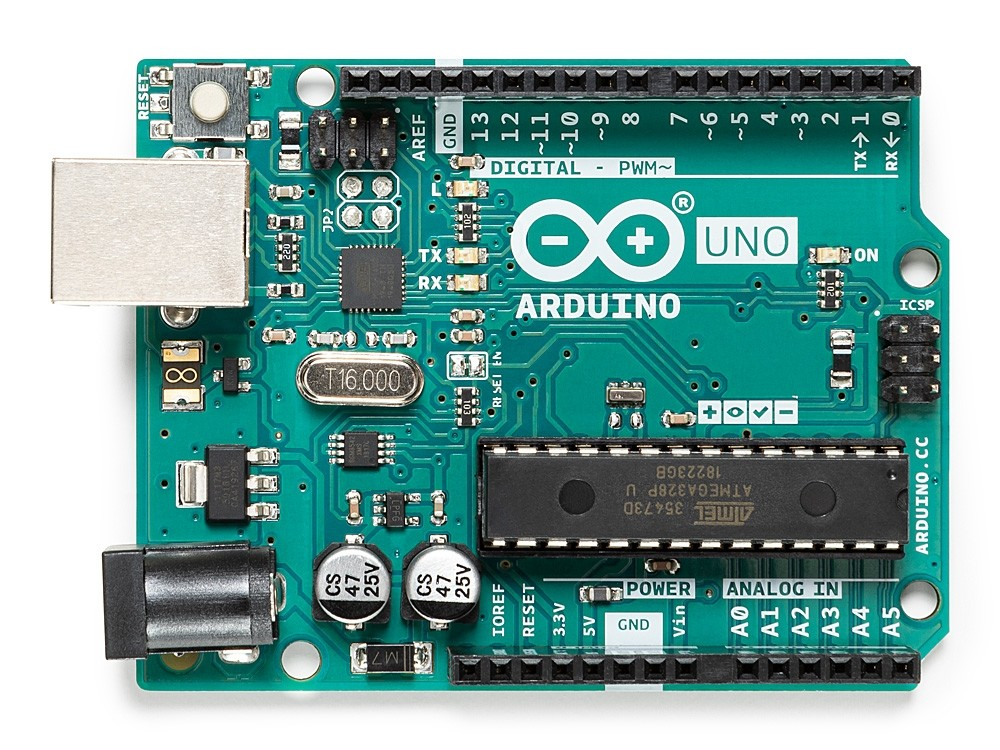
\includegraphics[width=0.3\textwidth]{ArduinoUNO.jpg}
    \caption{La carte Arduino UNO rev3 où la puce principale (longue et noire vers le bas à droite) est le MCU \href{http://ww1.microchip.com/downloads/en/DeviceDoc/Atmel-7810-Automotive-Microcontrollers-ATmega328P_Datasheet.pdf}{ATmega328P} avec des \href{https://www.circuito.io/blog/arduino-uno-pinout/}{ entrées/sorties} situées le long en haut et en bas de la carte alors que l'alimentation et un port USB sont sur la gauche. Photo provenant du \href{https://store.arduino.cc/usa/}{magasin en ligne} de la compagnie Arduino.}
    \label{fig:ArduinoUNO}
\end{figure}

\subsubsection*{Qu'est qu'un Arduino peut faire?}
Cela dépend des périphériques disponibles sur le MCU utilisé, soit ATmega328P de Atmel pour la carte Arduino UNO. Quelques exemples sont de l’acquisition de données, de la synchronisation de signaux, du traitement de données en temps réel, etc. Parmi les périphériques du MCU que l’Arduino utilise, deux (au minimum) seront utiles à la conception du système:
\begin{itemize}
    \item le \href{https://en.wikipedia.org/wiki/Analog-to-digital_converter}{convertisseur analogique-numérique} (\textit{analog-to-digital converter}, ADC) qui permet de lire une tension analogique, par exemple aux bornes d’une photorésistance ou celle qui était fournie par une pomme de terre au début du cours(!),
    \item le générateur de signaux en   \href{https://en.wikipedia.org/wiki/Pulse-width_modulation}{modulation de largeur d'impulsions} (\textit{pulse-width modulation}, PWM) qui permet de contrôler certains composants qui ne nécessitent pas un courant élevé, par exemple la base d’un transistor.
\end{itemize}

 Pour utiliser ces fonctionnalités, Arduino a implémenté des fonctions simples à utiliser, soit les fonctions \texttt{AnalogRead}  et \texttt{DigitalWrite/AnalogWrite}. Afin de faire l’acquisition d’un signal avec l’Arduino, les entrées qui sont identifiées \textbf{ADC} ou encore \textbf{A0, A1, A2,} … devront être utilisées. Pour générer un signal, les sorties qui sont identifiées \textbf{PWM} seront utilisées. Arduino, voulant simplifier la tâche, a indiqué que certaines entrées étaient dédiées à des fonctions spécifiques, mais en réalité, c’est le MCU qui décide ce qui se passe sur une entrée et plusieurs fonctions différentes peuvent être utilisées sur une seule et même entrée.
 
\subsubsection*{Comment utiliser un Arduino?}
Il faut le programmer, sauf que les MCU n'acceptent pas directement des langages interprétés de haut niveau\footnote{Des librairies se développent cependant dans plusieurs langages tels Python (\href{https://github.com/tino/pyFirmata}{pyFirmata}, \href{https://pypi.org/project/pyserial/}{pyserial}, ...) et \href{https://www.mathworks.com/help/supportpkg/arduinoio/examples/getting-started-with-matlab-support-package-for-arduino-hardware.html}{MATLAB} pour communiquer avec une carte Arduino à partir d'un ordinateur ou encore être exécutées directement sur d'autres types de MCU avec \href{https://www.digikey.ca/en/maker/blogs/2018/python-on-hardware}{CircuitPython} par exemple.}. Le C et le C++ sont les langages majoritairement utilisés pour cette programmation puisqu’ils sont rapides d’exécution tout en étant relativement simples à coder pour des langages compilés. Heureusement, la compagnie Arduino offre une \href{https://www.arduino.cc/en/software}{interface de programmation conviviale} qui contient déjà plusieurs fonctions "pré-codées" (\href{https://www.arduino.cc/en/Tutorial/BuiltInExamples}{
didacticiels ici}) et Tinkercad offre même en parallèle une \href{https://scientiffic.medium.com/tinkercad-circuits-code-blocks-9953d47b5a3f}{programmation visuelle avec des briques Scratch} si désiré. 

\noindent Quelques conseils avant de se lancer dans la programmation Arduino:
\begin{itemize}
    \item Toutes les variables doivent toutes être déclarées au début, ainsi que leur \href{https://en.wikipedia.org/wiki/C_data_types}{type} avant de les utiliser ailleurs dans le code.
    \item La fonction \texttt{void functionName()~\{\}} signifie seulement que la fonction ne retourne rien, car il faut aussi déclarer ce que la fonction retourne. Si la fonction retourne un entier, il faut plutôt écrire \texttt{int functionName()~\{\}}.
    \item L’intégralité de ce qui se passe lorsque l’Arduino exécute se trouve dans la fonction \texttt{loop()~\{\}}.
    \item Le code dans la fonction \texttt{setup()~\{\}} ne sera exécuté qu’une fois au démarrage de l’Arduino.
    \item Le moniteur série dans Tinkercad permet de faire des actions équivalentes à la commande \texttt{print} rencontrée en Python et bien d'autres langages; cela pourrait simplifier la tâche.
\end{itemize}

\subsection*{Photorésistance}
Une photorésistance est un composant électrique dont la résistance varie en fonction de l'irradiance, c'est-à-dire l’intensité lumineuse mesurée en \si[inter-unit-product=\ensuremath{{}\cdot{}}]{\watt\per\meter\squared}. Ces photorésistances sont fabriquées à partir de matériaux semiconducteurs dont la conductivité augmente lorsqu’ils sont exposés à la lumière. Par conséquent, la résistance de celles-ci varie à l'inverse de l'irradiance. La Figure~\ref{fig:photoresistance} montre la représentation de la photorésistance dans l’environnement Tinkercad.

\begin{figure}[h]
    \centering
    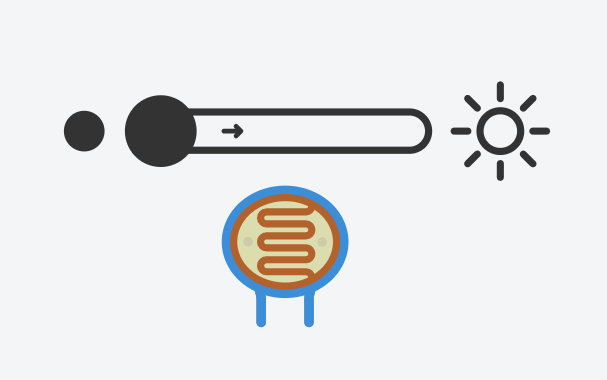
\includegraphics[width=0.4\textwidth]{Photoresistance.png}
    \caption{Photorésistance dans l’environnement Tinkercad. La glissière au-dessus permet d’ajuster l’irradiance en démarrant la simulation, puis en sélectionnant la photorésistance. Dans le cadre de ce projet de conception, la période du jour est représentée par la position de l’indicateur sur la glissière, avec la position la plus à gauche représentant la nuit.}
    \label{fig:photoresistance}
\end{figure}

\subsection*{Conseils d'utilisation de transistor}
Finalement, le.s transistor.s peut.vent être utilisé.s dans la conception du circuit pour contrôler une charge (le moteur DC) qui serait placée entre le collecteur et l'émetteur et alimentée par une tension $V_{CE}$. Le mode interrupteur, donné en exemple à la Figure~\ref{fig:InterrupteurMoteur}, ou le mode amplificateur peut être utilisé. La tension de contrôle $V_{BE}$ peut être générée par la carte Arduino UNO, ce qui permettrait d’adapter l’alimentation du moteur en fonction de la résistance d’une photorésistance qui pourra également être lue par l’Arduino.

%Refaire ce circuit avec des transistors à jonction bipolaire pour avoir une image avec RPM corrects. 
\begin{figure}[h]
    \centering
    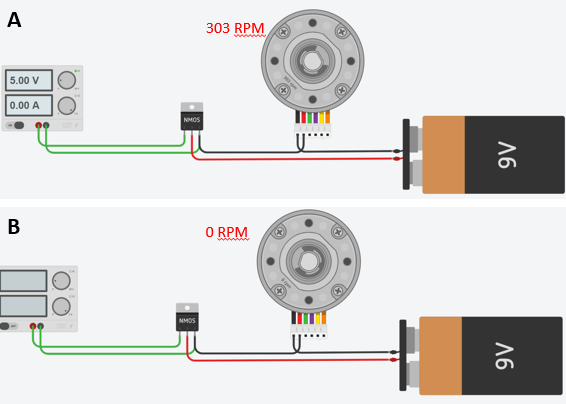
\includegraphics[width=0.35\textwidth]{InterrupteurMoteur.png}
    \caption{Moteur DC~437~RPM actionné en (A) puis éteint en (B) avec le transistor qui joue le rôle d'interrupteur. (A) Avec une tension de suffisante entre la base et l'émetteur du transistor, l’interrupteur est fermé et le courant circule entre la batterie de \SI{9}{\volt} et le moteur DC. (B) La base du transistor n'est plus sous tension et l'interrupteur est ouvert, d'où aucun courant ne circule dans le moteur.}
    \label{fig:InterrupteurMoteur}
\end{figure}

\end{document}
